\chapter{Current limits of EDMs}

The upper bounds of EDM measurements have been lowered over the last ~70 years as experiments reduce their statistical and systematical uncertainties in their \gls{edm} measurements of different atomic species and particles. Figure \ref{fig:EDMsearch} summarizes the uncertainties of the EDM measurements of the electron and neutron as well as atomic EDMs from Rd, Hg, and Xe.   

\begin{figure} [h!]
	\center
	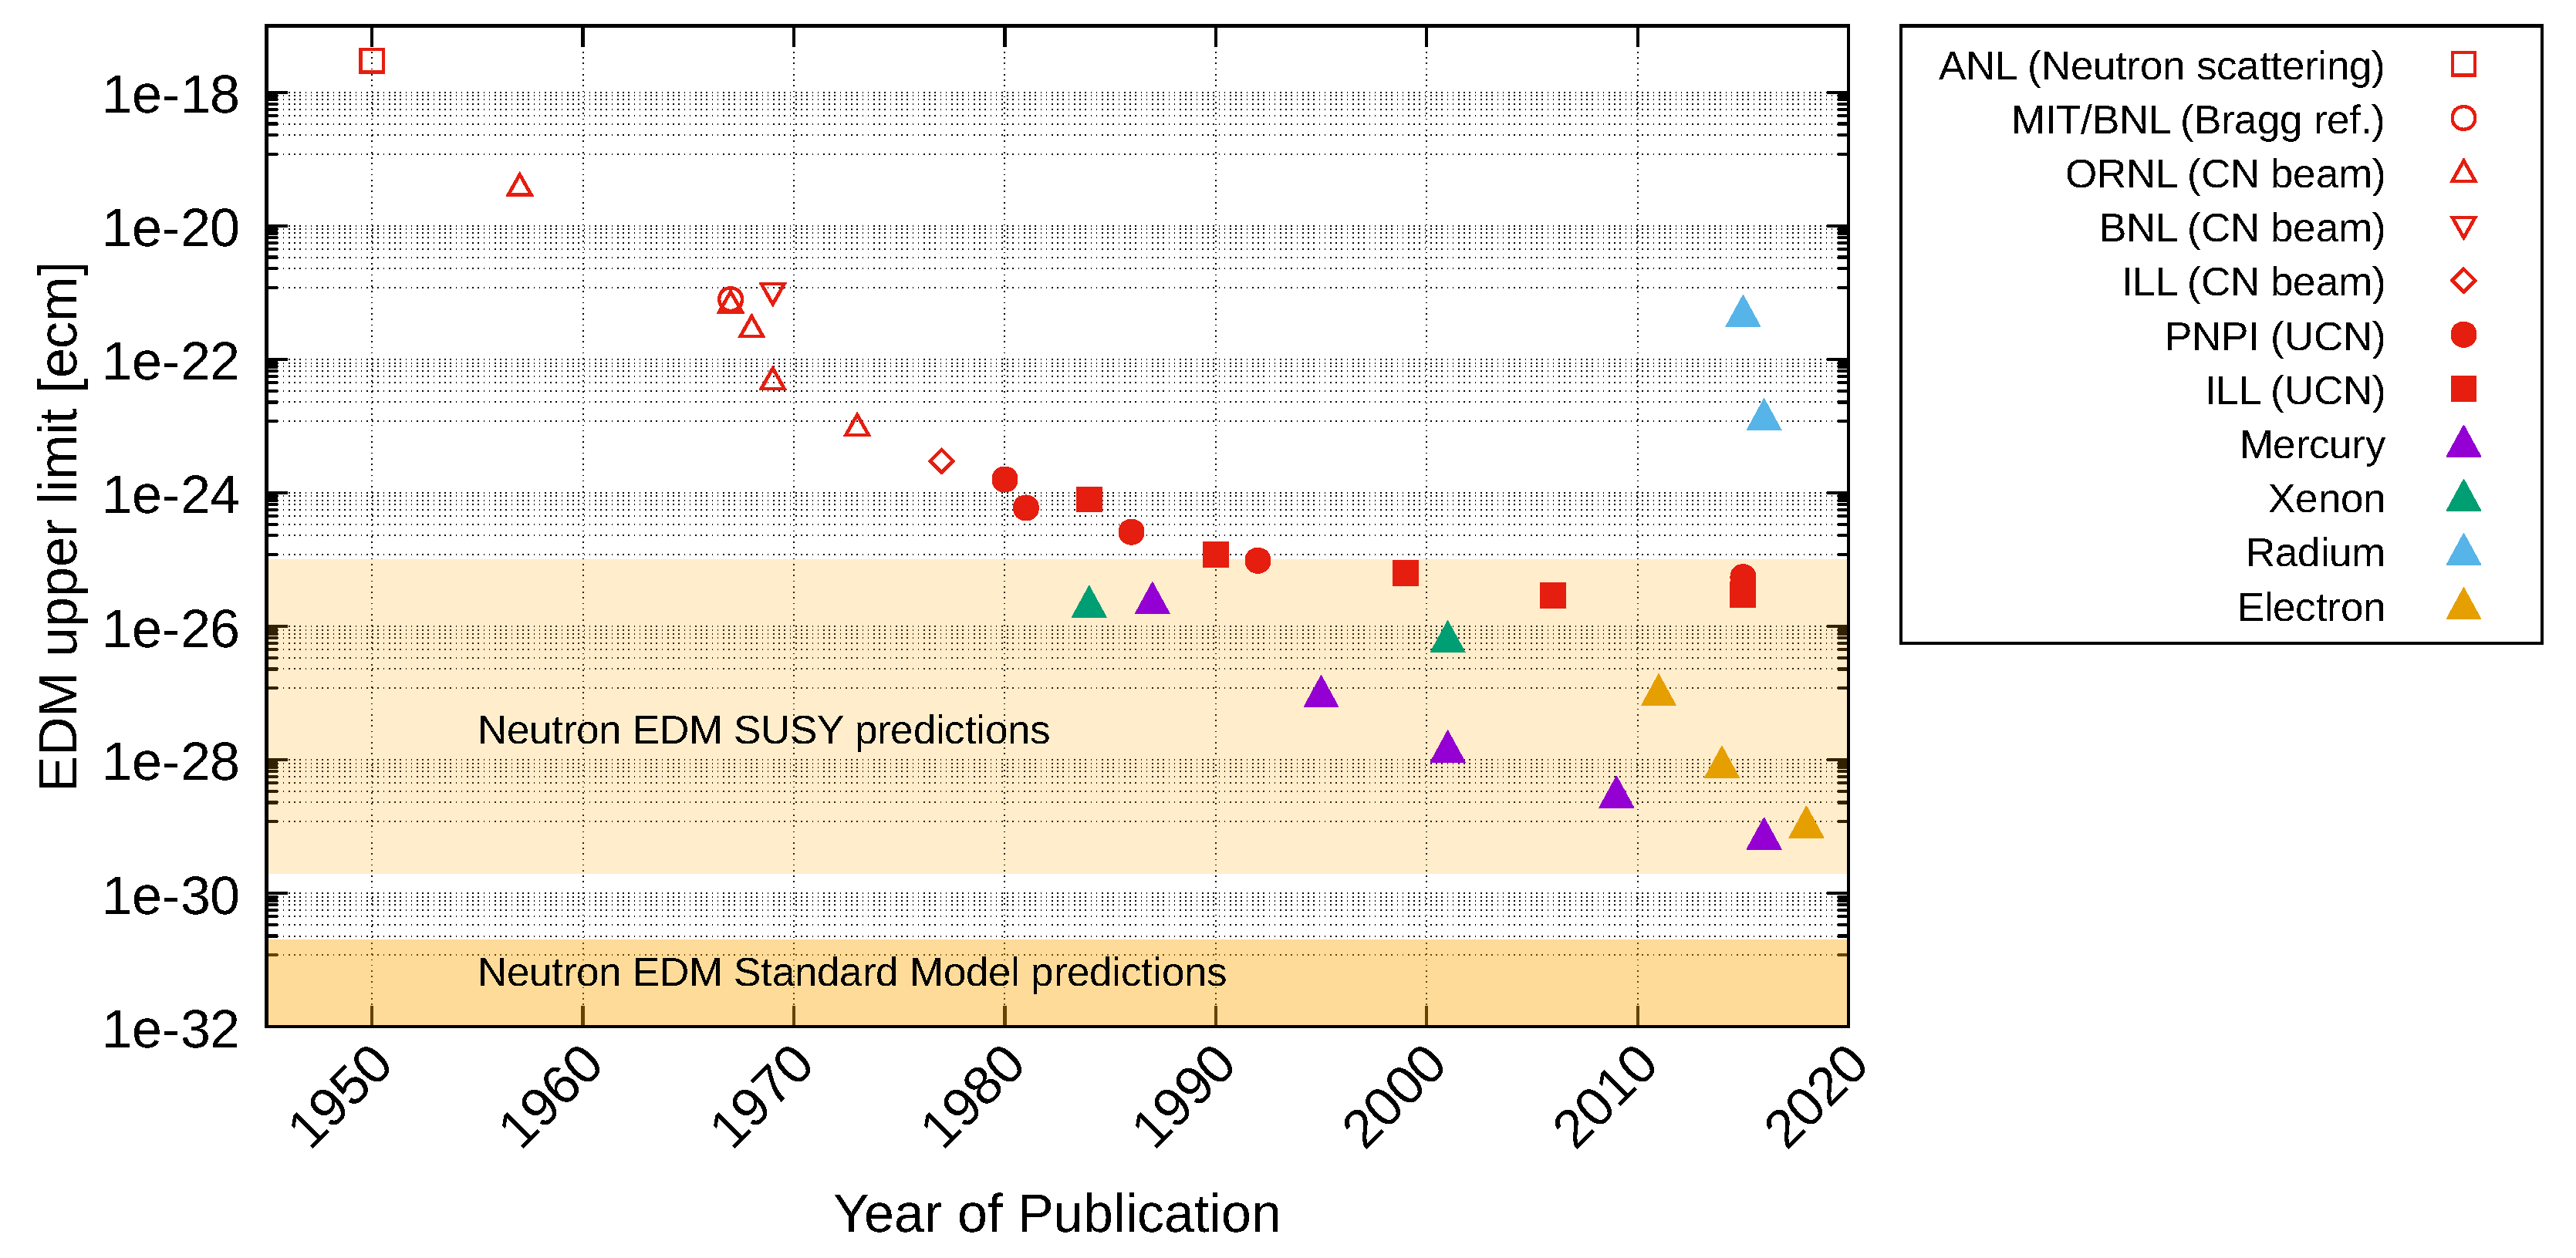
\includegraphics[width=.8\textwidth]{EDM-searches.png}
	\caption { The \gls{edm} measurements have been placing bounds that have been steadily going down over time,  as presented by Kuchler \cite{Kuchler}}.
		\label{fig:EDMsearch}
\end{figure}

The \gls{edm} predictions from beyond \gls{sm} physics are starting to be tested for the high energies interaction terms that contribute to EDMs at the TeV scale \cite{Chupp2015}. As the measured upper bound of $d_n$, $d_{^199\textrm{Hg}}$, and $d_{^199\textrm{Xe}}$ continue to be lowered from precision experiments, improved limits on beyond SM theories that have additional CP-violating physics are set. The search for EDMs play an important role probing new physics.